\section{An End-to-End Compression Framework Based
on Convolutional Neural Networks}

\begin{flushleft}
    \author{
    Feng Jiang, 
    Wen Tao, 
    Shaohui Liu, 
    Jie Ren, 
    Xun Guo, 
    Debin Zhao, 
    \emph{Member, IEEE}
    }
\end{flushleft}

\begin{center}
    \emph{IEEE TRANSACTIONS ON CIRCUIT AND SYSTEMS FOR VIDEO THECNOLOGY, VOL. 28, NO. 11, OCTOBER 2018}
\end{center}

\subsection{INTRODUCTION}
In recent years, within the field of computer vision, remarkable results have 
been achieved with regard to image compression. The purpose of compression 
is to be able to transmit, or save, the entire image at low bit rates. As far as 
decompression is concerned, deblocking and denoising techniques have been 
developed that are useful for obtaining good images. Further pre-processing 
steps have been found to negatively impact in system performance. Therefore 
the proposed method uses a framework composed of two convolutional 
networks (\emph{CNNs}). The first network, called compact convolutional neural 
newtork (\emph{comCNN}), is used for compression and uses the JPEG, JPEG2000 
and BPG encoding codecs. The second network, called reconstruction convolutional 
neural network (\emph{RecCNN}), is used for image decompression. A 
first example of the work carried out by the proposed framework is visible in 
the Fig. \ref{fig:output}.
\begin{figure}[h!]
    \centering
    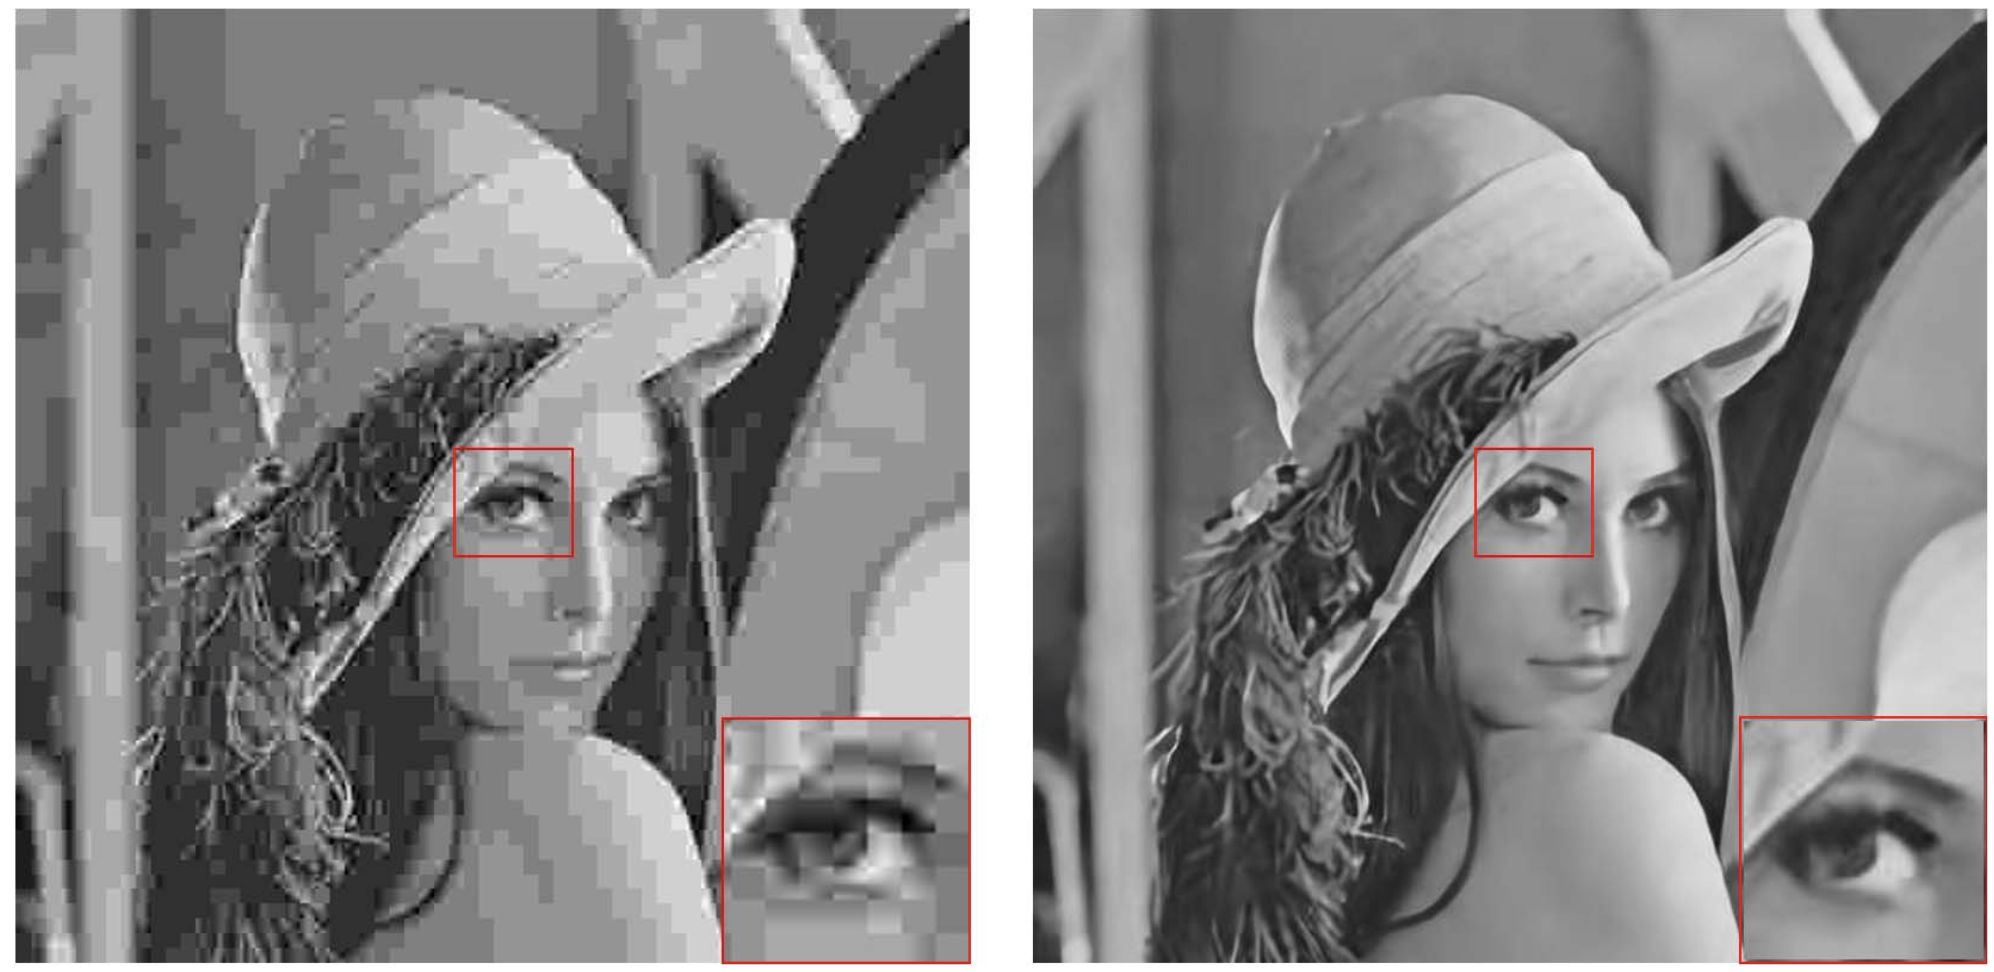
\includegraphics[width = 0.6 \linewidth]{images/paper3/output .png}
    \centering
    \caption{Left: the JPEG-coded image. Right: the decoded image.}
    \label{fig:output}
\end{figure}

\subsection{RELATED WORK}
\subsubsection{Image Deblocking and Artifacts Reduction}
Going back to talking about the deblocking technique, this is useful for removing 
all those blocks that visually worsen the appearance of each image. 
The various restoration techniques model the distortion created in the compression 
phase in order to reduce artifacts. Many methods already proposed 
in the state of the art use techniques that have a great impact on performance 
when they adopt iterative restoration processes. Therefore, the proposed 
method tries to obtain the same result but with a lower computational 
cost.

\subsubsection{Image Super-Resolution Based on Deep Learning}
Convolutional neural networks (\emph{CNNs}) have been used for super resolution 
(\emph{SR}) images especially when residual learning and gradient-based optimization 
algorithms have been proposed to train a deep network. According to 
some studies, the depth of a network doesn't always lead to good performance. 
Other researchers, on the other hand, claim the opposite.

\subsubsection{Image Compression Based on Deep Learning}
Deep learning was used for lossy and loseless compressions achieving good 
performance. There have been some methods that have prevailed over others. 
However, all of these methods ignore compatibility with various image codecs, 
thus limiting their use in some existing systems. The proposed framework 
solves this problem by operating with different image codecs, also taking into 
account the compression performance.

\subsection{THE PROPOSED COMPRESSION FRAMEWORK}
\subsubsection{Architecture of End-to-End Compression Framework}
\begin{figure}[htbp]
    \centering
    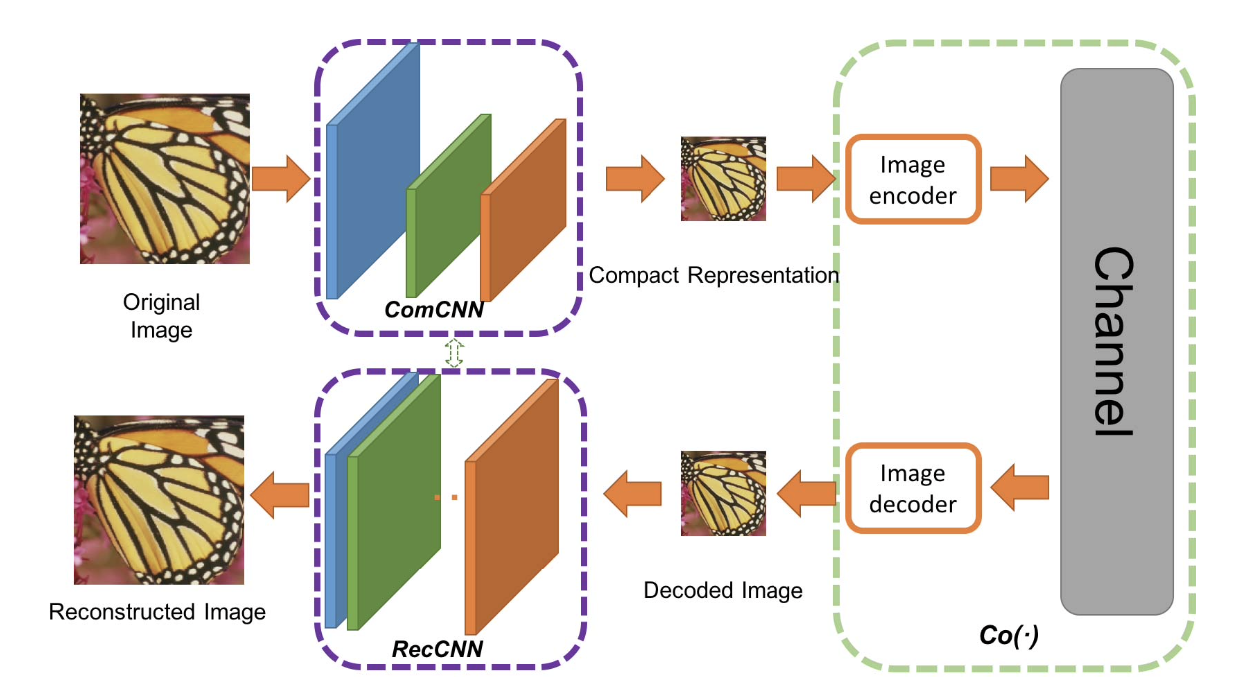
\includegraphics[width = 0.8 \linewidth]{images/paper3/framework.png}
    \centering
    \caption{The proposed novel compression framework.}
    \label{fig:framework}
\end{figure}
As mentioned, the first \emph{ComCNN} convolutional network is used to generate 
a compact representation of the input image which preserves the structural 
information and facilitates the reconstruction of image in high quality. The 
second convolutional network, \emph{RecCNN}, is used to improve the quality of the 
decoded image. In particular:
\begin{enumerate}
    \item \emph{Compact Representation Convolutional Neural Network (ComCNN)}: 
    This network is made up of three weighted layers. The first layer is 
    used to perform the extraction and representation of patches from the 
    input image. 64 filters are used, each 3x3xc in size where c indicates 
    the number of image channels. Thanks to these filters, 64 feature maps 
    are generated. The second layer has the task of downscaling and improving 
    the features with convolutional operations having stride equal to 2 
    and 64 filters of 3x3x64 size. In the last layer, \emph{c} filters, of 3x3x64 
    size, are used to reconstruct the compact representation.
    \item \emph{Reconstruction Convolutional Neural Network (RecCNN)}: The layers 
    are identical to those of the \emph{ComCNN} network, unlike the number. To 
    speed up training, as well as performance, methods such as residual 
    learning and batch normalization \cite{0799924133} are used. Finally, the image will 
    be upsampled to its original size, using a cubic interpolation.
\end{enumerate}

\subsubsection{Learning Algotrithm}
In order for both networks to have good training, their parameters must be 
optimized (weights and bias). To achieve this, the following formulas will 
have to be optimized iteratively:
\begin{equation}
    \hat{\theta_1} = \argmin\limits_{\theta_1}||Re(\hat{\theta_2},Cr(\theta_1,x))-x||^2
\end{equation}
\begin{equation}
    \hat{\theta_2} = \argmin\limits_{\theta_2}||Re(\hat{\theta_2},\hat{x}_m)-x||^2
\end{equation}
Where:
\begin{itemize}
    \item \emph{x} represents the original image
    \item $ \hat{\theta_1} $ and $ \hat{\theta_2} $ are the parameters of \emph{ComcCNN} and \emph{RecCNN}
    \item $ C_r(\cdot) $ and $ R_e() $ represent the \emph{ComcCNN} and \emph{RecCNN}
    \item $ \hat{x}_m $ is th e decoded compact representation of \emph{x}
\end{itemize}

\subsubsection{Loss Functions}
For ComCNN training: as a loss function, we use the mean square error (\emph{MSE}):
\begin{equation}
    L_1(\theta_1) = \frac{1}{2N}\sum_{k=1}^N||Re(\hat{\theta_2}, C_r(\theta1,x_k))-x_k||^2
\end{equation}
Where \emph{N} and $ \theta_1 $ represent the batch size and the trainable parameter.
For REcCNN training: after obtaining a set of compact $ x_m $ images from 
\emph{ComCNN} and the original \emph{x} images, we also use the mean square error 
(\emph{MSE}) here:
\begin{equation}
    L_2(\theta_2) = \frac{1}{2N}\sum_{k=1}^N||res(Co(\hat{x}_{mk}), \theta_2) - (Co(\hat{x}_{mk})-x_k)||^2
\end{equation}
Where $ \theta_2 $ are the trained parameters of the network while $ res(\cdot) $ represent 
the residual learning of the \emph{RecCNN}.

\subsection{EXPERIMENTS}
In order to evaluate the performance of the proposed framework, the results 
obtained were compared with six deblocking methods and two denoising 
methods. In order to train the network, the \emph{MatConvNet} \cite{0799924138} package is 
used.

\subsubsection{Datasets for Training and Testing}
For training, 400 images of 180x180 size are used. The patches used are in 
total 204800 $ (400x8x64)^2 $, with stride equal to 20. For the test, however only 
7 images are used which obviously are not present in the training ones.

\subsubsection{Model Initialization}
The initialization of the weights takes place following the method in \cite{0799924140}, 
while for the optimization of the gradient the method defined in \cite{0799924121} is used.
The training of the ComCNN network takes place in 50 epochs with a batch 
size of 128. The learning rate falls from 0.01 to 0.0001. The initial parameters 
of the second RecCNN network are identical to those of the first network, 
including the batch size.

\subsubsection{Experimental Results}
Various quality factors (\emph{QS}), useful for indicating the degree of loss in a 
compressed image, are manually set in order to achieve the same bits per 
pixel (\emph{bpp}) of the original image. In order to compare the other methods 
existing at the state of the art with the proposed method, two compression 
quality indices were used such as \emph{PSNR} and \emph{SSIM}. With a \emph{QF} set to 5 and 10, the 
comparison results obtained are shown in figure \ref{fig:QF5}.
\begin{figure}[htbp]
    \centering
    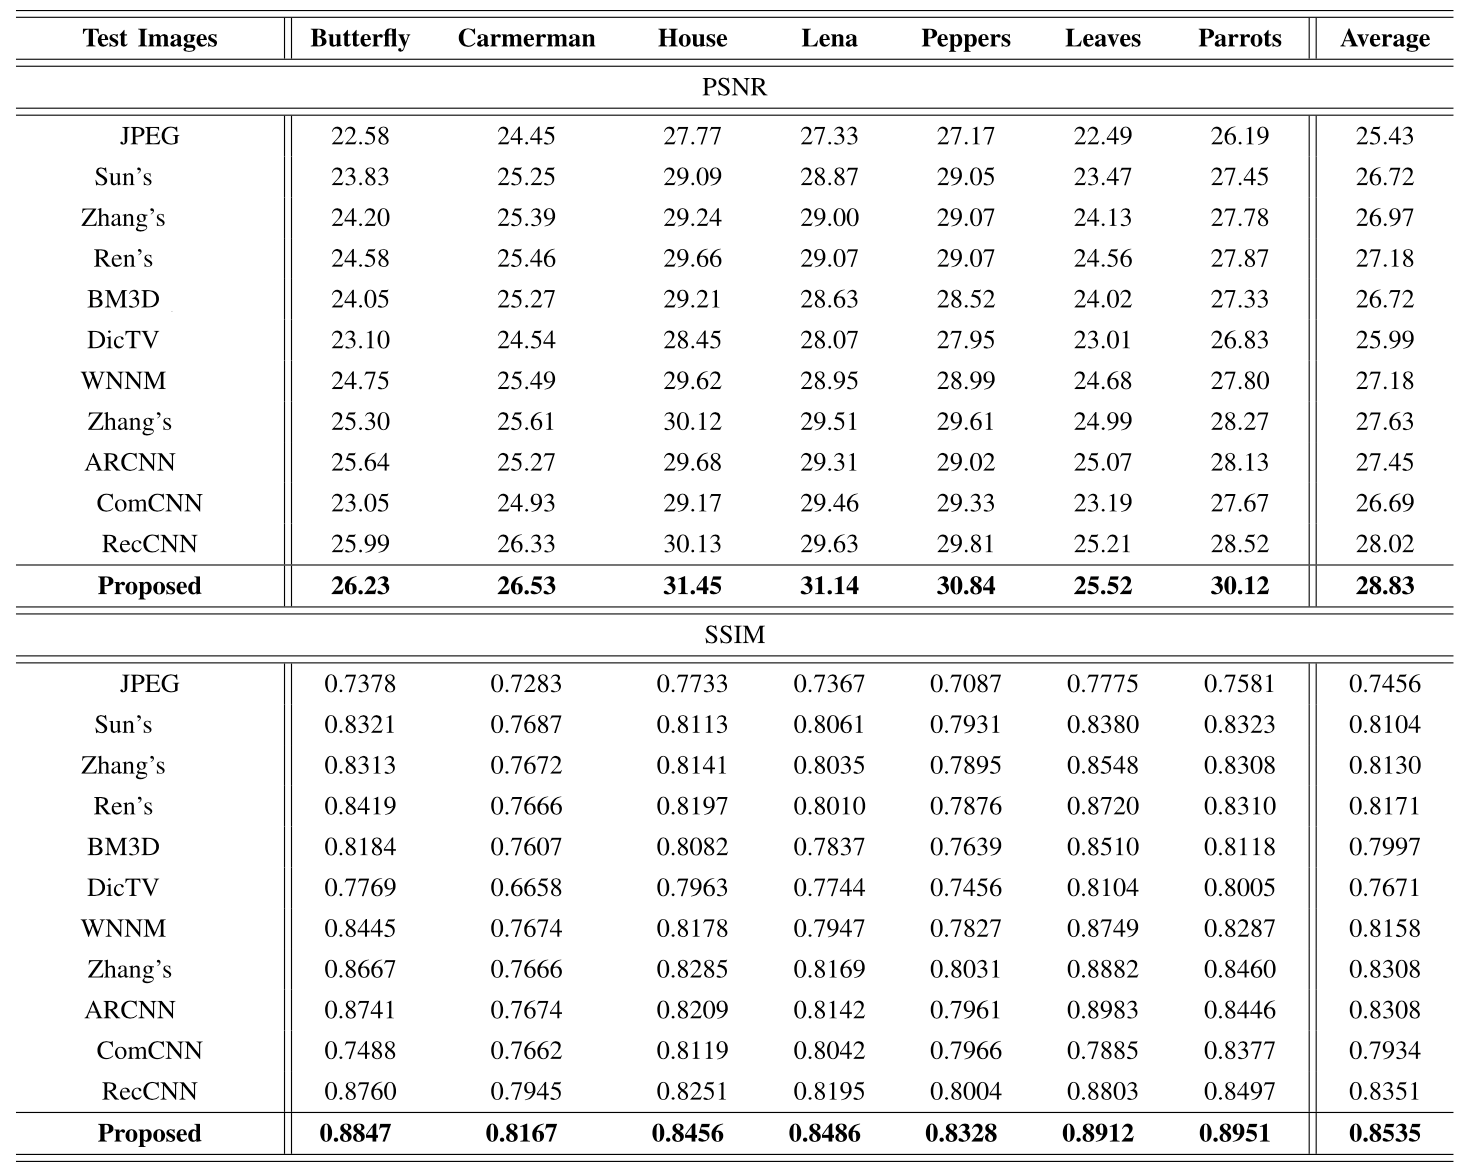
\includegraphics[width = 1 \linewidth]{images/paper3/comparison.png}
    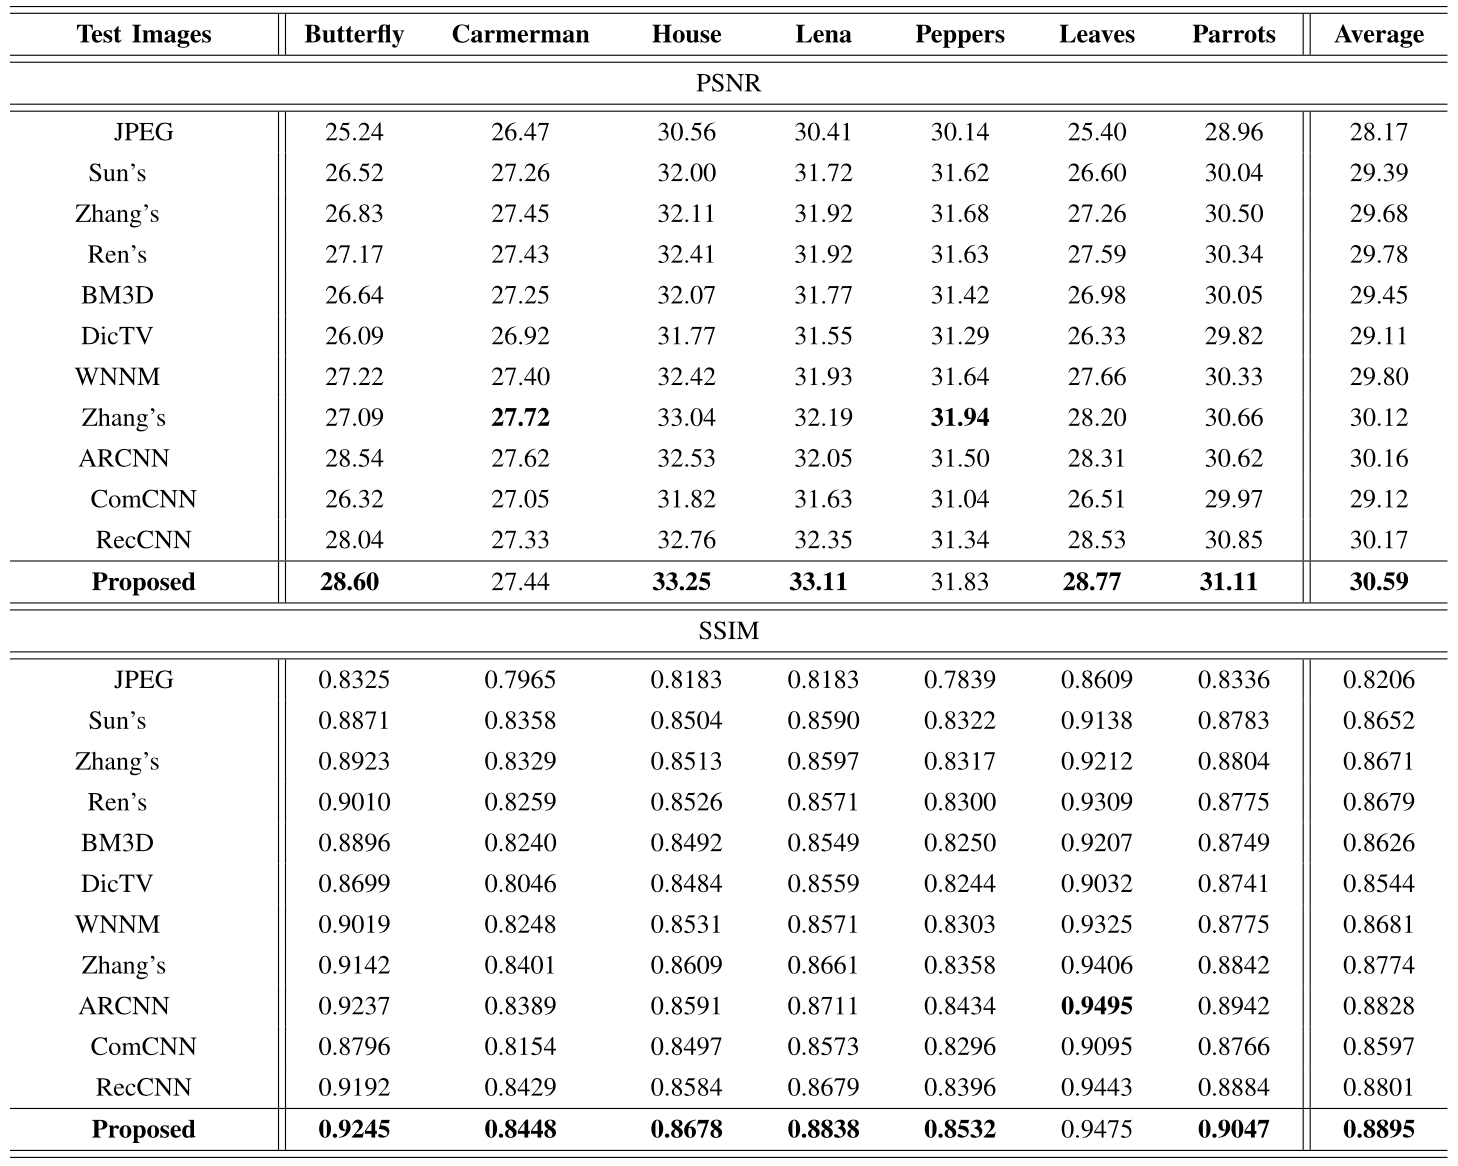
\includegraphics[width = 1 \linewidth]{images/paper3/comparison2.png}
    \centering
    \caption{JPEG: QF=5 and QF=10, PSNR(db) and SSIM results of alghoritms image deblocking and denoising.}
    \label{fig:QF5}
\end{figure}
As we can see from figure \ref{fig:QF5}, 
the most used method in the state of the art \cite{0799924108} blurs the image a lot by 
losing some detail on the corners, the proposed method has a gain of 1.20db 
in PSNR, producing compressed images with better quality, and a gain of 
0.0227 in SSIM indicating a high similarity with the original image. The 
proposed framework also manages to exceed the performance of the ARCNN 
\cite{0799924109} method which represents a milestone in this area. The strength of the 
proposed method is based on obtaining better compression than commonly 
used codecs, such as \emph{JPEG}, \emph{JPEG2000} and \emph{BPG}, in a variable bit rate 
range. As we can see from the comparison made in figure \ref{fig:JPEG2000p}, the difference 
in visual quality between the proposed method and the JPEG2000 codec 
is considerable. With the same amount of bit rates, the JPEG2000 codec 
produces worse results by losing several structural information.
\begin{figure}[htbp]
    \centering
    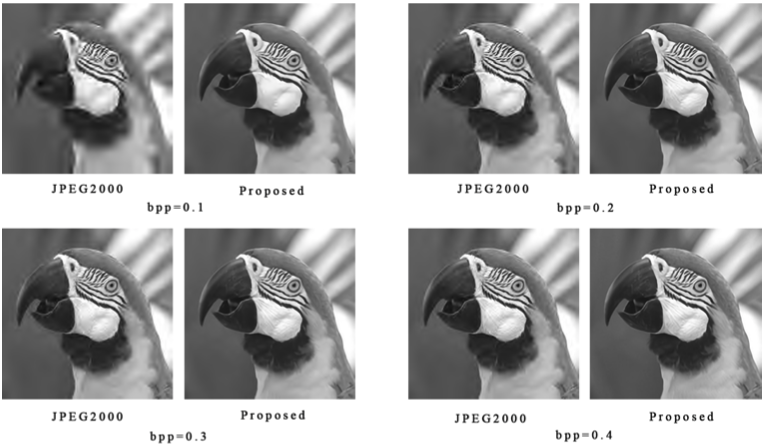
\includegraphics[width = 1 \linewidth]{images/paper3/JPEG2000p.png}
    \centering
    \caption{Performance comparison of JPEG2000 at difference bit rates.}
    \label{fig:JPEG2000p}
\end{figure}
\begin{figure}[htbp]
    \centering
    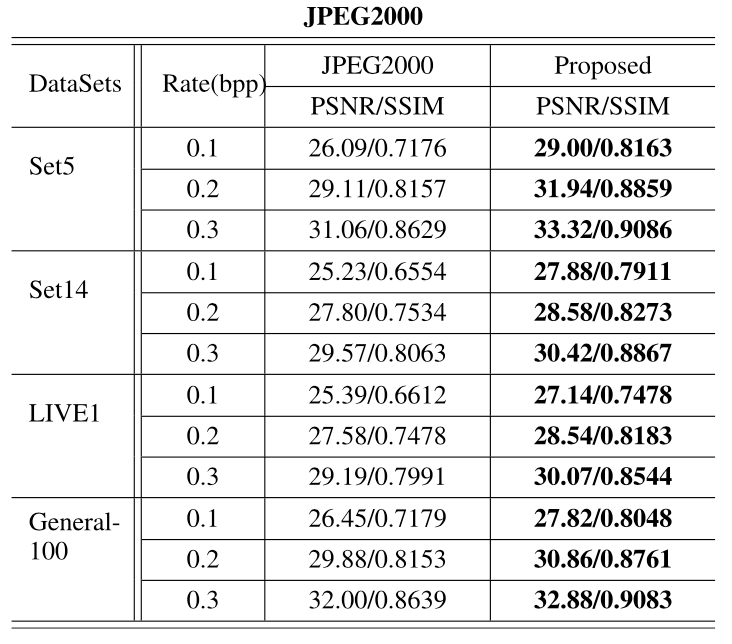
\includegraphics[width = 0.6 \linewidth]{images/paper3/JPEG2000.png}
    \centering
    \caption{Average PSNR(dB)/SSIM results of JPEG2000 and the proposed method.}
    \label{fig:JPEG2000}
\end{figure}
As for the BPG codec, 
if used in combination with the ComCNN and RecCNN networks, it reaches 
higher PSNR and SSIM levels than when used individually or with only one 
of the two networks, moreover, on average, it has a saving of about 5.22\% of 
the amount of bit rate.
\begin{figure}[htbp]
    \centering
    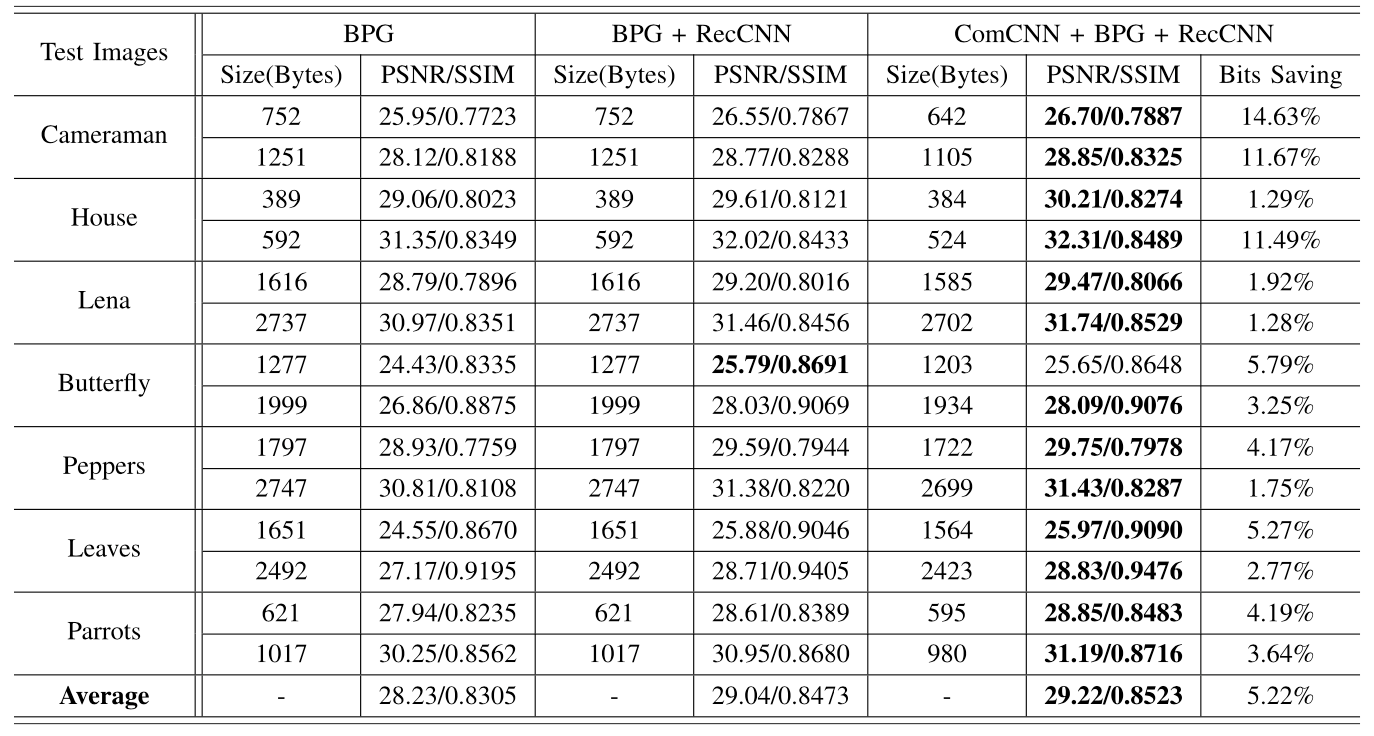
\includegraphics[width = 1 \linewidth]{images/paper3/BPG.png}
    \centering
    \caption{BPG: PSNR (dB) and SSIM result of BPG, BPG + RecCNN and the proposed method.}
    \label{fig:BPG}
\end{figure}

\subsubsection{Running Time}
The execution time of all algorithms, CPU and GPU, are shown in figure \ref{fig:time}. 
It should be noted that the time reached by the GPU was calculated only 
for the proposed method. The processed images, in grayscale, are in a size 
of 256x256. The proposed algorithm appears to be the fastest compared to 
the others.
\begin{figure}[htbp]
    \centering
    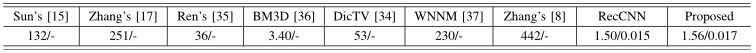
\includegraphics[width = 1 \linewidth]{images/paper3/time.png}
    \centering
    \caption{Running time(s) of compared methods in CPU (/GPU) }
    \label{fig:time}
\end{figure}

\subsection{CONCLUSION}
The proposed method seems to have the best performance compared to other 
methods already existing in the state of the art. The proposed technique 
then validates the use of one or more convolutional neural networks to carry 
out the task of encoding and decoding images, even in some cases achieving 
better quality than existing codecs for image compression.